\section{Background on Function Approximation with Neural Networks}
\label{sec:apx:background}
In this paper, we consider the approximation of target functions $f:\R^n\to\R$ that are
continuous on a bounded set $\Bc\subset\R^n$ containing the origin, which we denote as $f\in 
\Cs(\Bc)$.

Formally, for a given target function $f\in \Cs(\Bc)$, positive integer $N\in\N$, and positive 
scalar $\epsbase>0$ (which may depend on $N$) there exists some vector $\theta\in\R^N$ and 
nonlinear, continuous almost everywhere basis functions $\Bs_1,\dots,\Bs_N:\R^n\to\R$ such that 
the approximation
\begin{equation}\label{eq:apx:genApx}
\fh(x) \ := \ \sum_{i=1}^N \theta_i\,\Bs_i(x)
%\approx f(x) \hspace{40pt}\forall x\in\Bc
\end{equation}
satisfies
\begin{equation}\label{eq:apx:normBound}
%\sup_{x\in\Bc}\abs{f(x)-\fh(x)} \leq \epsbase
%\qquad\text{or}\qquad
\normB{\fch(x)-\fh(x)} \ \leq \ \epsbase \ \ .
\end{equation}
Here, we denote the the $L_2(\Bc,\muB)$ norm
$$
\normB{\fch(x)} \ := \ \left(\int_B|\fch(x)|^2\,\muBdx\right)^{\frac{1}{2}}
$$
with $\muB$ as the uniform probability measure over $\Bc$ such that $\int_\Bc\muBdx=1$, and some
\textit{affine shift} $\fch(x)=f(x)-\mathscr{a}^\top\!x -\mathscr{b}$, for some 
$\mathscr{a}\in\R^n$ and $\mathscr{b}\in\R$.
% (typically $\mathscr{a}=\nabla f(0)$ and $\mathscr{b}=f(0)$).

We will assume that the basis function is parameterized $\Bs(x\,;\upgamma)$ and is a 
composition of some nonlinear, continuous almost everywhere function $\sigma:\R\to\R$ together
with an affine transformation of $\R^n$ into $\R$ according to the \textit{parameter} 
$\upgamma\in\Upsilon$. We define each point $\upgamma:=[w^\top\ b]^\top=[w_1\ \dots\ w_n\ 
b]^\top$ with $w\in\R^n\setminus\{0_n\}$ as the \textit{weight vector} and $b\in\R$ as the
\textit{bias term}. We assume the \textit{parameter set} $\Upsilon$ is a bounded subset of 
$\R^n\setminus\{0_n\}\times\R$. And so, we set $\Bs(x\,;\upgamma_i)=\sigma(w_i^\top 
x+b_i)=\sigma(\pariX)$, where 
$X:=[x_1\ \cdots\ x_n\ 1]^\top$ and we denote $\upgamma_i=[w_i^\top\ b_i]^\top=[w_{i,1}\
\dots\ w_{i,n}\ b_i]^\top$, for all $i\in[N]$. 

We will use the term \textit{base approximation} to define, for some vector $\theta\in\R^N$ and
\underline{fixed} parameters $\upgamma_1,\dots,\upgamma_N\in\Upsilon$, for any integer $N\in\N$,
the sum
\begin{equation}\label{eq:apx:baseApx}
\fhN(x) = \sum_{i=1}^{N} \theta_i\,\sigma(\pariX)
%\approx f(x) 
%\hspace{40pt}\forall x\in\Bc
\ \ ,
\end{equation}
and \textit{random approximation} to define, for
% is similarly constructed, but in this case the parameters are
%\textit{randomly sampled} from $\Upsilon$. Thus, it refers 
some vector $\vartheta\in\R^R$ and \textit{randomly sampled} parameters
$\upgammab_1,\dots,\upgammab_R\in\Upsilon$, for any integer $R\in\N$, the sum
\begin{equation}\label{eq:apx:rndApx}
\fhR(x\,;\upgammab_1,\dots,\upgammab_R) = \sum_{j=1}^{R}\vartheta_j\,\sigma(\parbjX)
%\approx f(x) \hspace{40pt}\forall x\in\Bc
\ \ .
\end{equation}
%Note that we use integer $R$ and index $j$ for random approximations to distinguish them
%from base approximations, but otherwise there is no significance.

Note that these linear combinations are equivalent to a feedforward 
neural network with a single hidden layer, as depicted in Figure~\ref{fig:apx:SHLNN}, wherw 
$x_0=1$. Hence why we refer to $\sigma$ as an \textit{activation function}, as the output of 
each neuron is the activation of the weighted inputs (plus bias term) to the neuron. We will 
assume that the activation function $\sigma$ is bounded (growth)
% over all feasible inputs$\parX$ in $\Upsilon\times\Bc\times\{1\}$, 
as follows.

\begin{figure}
\centering
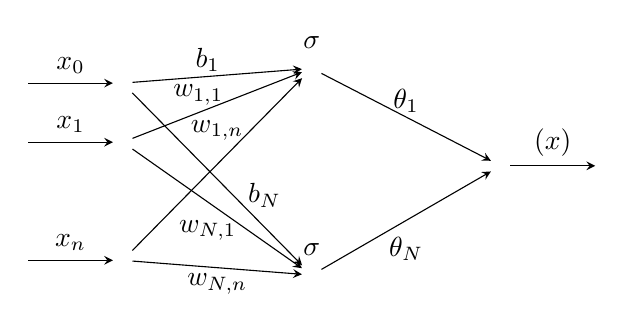
\begin{tikzpicture}[x=1.2cm, y=0.75cm, >=stealth]

\foreach \m/\l [count=\y] in {1,2,missing,3}
  \node [every neuron/.try, neuron \m/.try] (input-\m) at (0,1.5-\y) {};

\foreach \m [count=\y] in {1,missing,2}
  \node [every neuron/.try, neuron \m/.try ] (hidden-\m) at (2,2.5-\y*1.75) {};

\foreach \m [count=\y] in {1}
  \node [every neuron/.try, neuron \m/.try ] (output-\m) at (4,0.1-\y) {};

%\foreach \l [count=\i] in {1}
%  \draw [<-] (input-\i) -- ++(-1,0)
%    node [above, midway] {$x_\l$};

\foreach \l [count=\i] in {0,1,n}
  \draw [<-] (input-\i) -- ++(-1,0)
    node [above, midway] {$x_\l$};

\foreach \l [count=\i] in {1,n}
  \node [above] at (hidden-\i.north) {$\sigma$};

\foreach \l [count=\i] in {1}
  \draw [->] (output-\i) -- ++(1,0)
    node [above, midway] {$\fh(x)$};

\foreach \i in {1,...,3}
  \foreach \j in {1,...,2}
    \draw [->] (input-\i) -- (hidden-\j);

\foreach \i in {1,...,2}
  \foreach \j in {1}
    \draw [->] (hidden-\i) -- (output-\j);

%\foreach \l [count=\x from 0] in {Input, Hidden, Ouput}
%  \node [align=center, above] at (\x*2,2) {\l \\ layer};

\node[] at (0.9,0.9) {$b_1$};
\node[] at (1.5,-1.4) {$b_N$};
\node[] at (0.8,0.3) {$w_{1,1}$};
\node[] at (1.0,-0.3) {$w_{1,n}$};
\node[] at (0.9,-2.0) {$w_{N,1}$};
\node[] at (1,-2.9) {$w_{N,n}$};
\node[] at (3,0.2) {$\theta_1$};
\node[] at (3,-2.3) {$\theta_N$};

\end{tikzpicture}
\caption{\label{fig:apx:SHLNN} Single hidden-layer neural network with $\sigma$ activation 
function.}
\end{figure}


\begin{assumption}\label{sigAsmpt}
\textit{
The nonlinear, continuous almost everywhere activation function $\sigma:\R\to\R$ is bounded 
(growth) over all feasible inputs, such that either of}
\begin{enumerate}
\item $|\sigma(u) - \sigma(v)| \ \leq \ \Dsig$
\item $|\sigma(u) - \sigma(v)| \ \leq \ \Lsig\,|u-v|$
\end{enumerate}
\textit{
hold for all $u,v\in\Ic:=\{\parX \ | \ (\upgamma,X)\in\Upsilon\times\Bc\times\{1\}\}$,
with positive scalar $\Dsig$ or $\Lsig$.}
\end{assumption}

If we shift the activation to the origin as $\sigmach(y):=\sigma(y)-\sigma(0)$, this maintains 
the assumption with the same constant in either case.
The (scaled) step function $\sstep$ and the ReLU function $\relu$, defined as
\begin{align}
\sstep(y) &= 
\begin{cases*}\label{eq:pe:step}
0 \quad\text{if } y\leq0 \\
c \quad\text{if } y>0
\end{cases*}
\qquad \text{(scaled step)} \\
\relu(y) &= 
\begin{cases*}\label{eq:pe:ReLU}
0 \quad\text{if } y\leq0 \\
y \quad\text{if } y>0
\end{cases*}
\qquad \text{(ReLU)} \ \ ,
\end{align}
are examples meeting Assumption~\ref{sigAsmpt}, with $\Dsig=c$ and $\Lsig=1$ respectively,
where $c>0$ is an arbitrary positive scalar.